\chapter{Inside Sin}
\restartlist{enumerate}
\begin{enumerate}
	\item \formation{\tidus}{\lulu}{\rikku}
	\item Walk along the path
	\item Charge \tidus, \lulu\ and \rikku\ \od
	\item Charge \yuna\ \od\ if you haven't done it yet
	\liteversiondetermination{Exclude}{%
		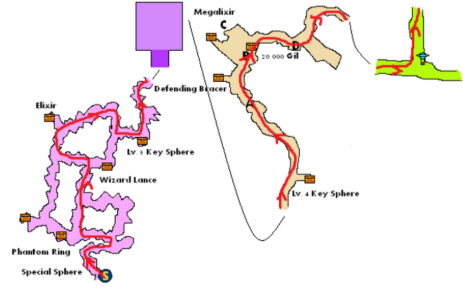
\includegraphics{graphics/sinpath}
		\item Go up the steps, \sd
	}
\end{enumerate}
\begin{battle}[80000]{Seymour Omnis}
	\begin{itemize}
		\rikkuf Mix 2x Wings to Discovery
		\tidusf Slice and Dice (Intentionally Fail)
		\luluf Thunder Fury (6 hits required)
	\end{itemize}
\end{battle}
\begin{enumerate}[resume]
	\liteversiondetermination{Exclude}{\item \sd, walk north.}
	\item Charge \tidus, \lulu\ and \rikku\ \od
	\item Charge \yuna\ \od\ if you haven't done it yet
	\liteversiondetermination{Exclude}{\item Turn left onto the bridge, go onto the next screen.}
	\item Heal everyone except \rikku. \important{Rikku must remain in critical HP for the BFA fight.}% using the \rikku command raises an error
	\liteversiondetermination{Exclude}{\item Complete the minigame, picking up the eggs and avoiding the crystals.}
\end{enumerate}
\liteversiondetermination{Exclude}{%
\begin{enumerate}[resume]
	\item Walk up to Jecht, \cs[4:30]
\end{enumerate}
}
\vfill\ \colbreak
\begin{battle}[180000]{Braska's Final Aeon}
	\begin{itemize}
		\tidusf Talk
		\switch{\yuna}{\rikku}, Use Chocobo Feather on \tidus
		\switch{\auron}{\yuna}, Switch Weapon
		\rikkuf Switch Weapon
		\switch{\yuna}{\lulu}, Switch Weapon
		\rikkuf Mix 2x Wings to Discovery
		\tidusf Talk
		\switch{\lulu}{\kimahri}, Lancet
		\tidusf Slice and Dice
		
		\vspace{\baselineskip}

		\switch{\rikku}{\yuna}, Grand Summon Shiva
		\shivaf Diamond Dust
		\switch{\kimahri}{\rikku}, Use Fire Gem
		\switch{\tidus}{\lulu}, Thunder Fury (7 Hits Required)
	\end{itemize}
\end{battle}
\colend
\liteversiondetermination{Exclude}{%
\begin{enumerate}[resume]
	\item \cs+\skippablefmv[4:00]
\end{enumerate}
}
\begin{battle}{Possessed  Aeons}
	In the Aeon fights you need up to 4 poison fangs. If you have 2 or fewer Poison Fangs prioritise using them on Ifrit and Ixion.
	\begin{itemize}
		\valeforf Throw Poison Fang (or 2x Bomb Core / Lightning Marble / Arctic Wind / Dream Powder if short on Poison Fangs)
		\ifritf Throw Poison Fang + any non-fire throwable
		\ixionf Throw Poison Fang + any non-lightning throwable
		\shivaf Throw Poison Fang (or 2x Bomb Core / Lightning Marble / Arctic Wind / Dream Powder if short on Poison Fangs)
		\bahamutf
			\begin{itemize}
				\rikkuf Throw Bomb Core / Lightning Marble / Arctic Wind / Dream Powder
				\switch{\yuna}{\kimahri}
				\kimahrif Self Destruct
			\end{itemize}
	\end{itemize}
\end{battle}
\liteversiondetermination{Exclude}{%
\begin{enumerate}[resume]
	\item \cs[1:40]
\end{enumerate}
}
\begin{battle}[99999]{Yu Yevon}
	\begin{itemize}
		\item \rikku\ Zombiestrike Weapon:
			\begin{itemize}
				\rikkuf Attack
				\item Anyone Throw Phoenix Down at Yu Yevon
			\end{itemize}
		\item \lulu\ Zombiestrike Weapon:
			\begin{itemize}
				\rikkuf Switch Weapon
				\luluf Attack
				\rikkuf Throw Phoenix Down at Yu Yevon
			\end{itemize}
		\item \kimahri\ Zombiestrike Weapon:
			\begin{itemize}
				\rikkuf Switch Weapon
				\kimahrif Attack
				\item Anyone Throw Phoenix Down at Yu Yevon
			\end{itemize}
		\item Anyone Else Zombiestrike Weapon:
			\begin{itemize}
				\switch{\rikku}{character with Zombie Strike Weapon}
				\item That Character: Attack
				\item Anyone Throw Phoenix Down at Yu Yevon
			\end{itemize}
		\item \rikku\ Zombietouch Weapon:
			\begin{itemize}
				\rikkuf Switch Weapon to Zombietouch Weapon
				\luluf Switch Weapon
				\rikkuf Attack
				\luluf If Curaga deals 9999 damage to Yu Yevon (White numbers) Throw Phoenix Down at Yu Yevon, otherwise Switch Weapon
				\item Keep switching weapon on \lulu\ and \kimahri\ until \rikku\ lands Zombie status and the curaga numbers are white
				\item Once curaga lands, anyone Throw Phoenix Down at Yu Yevon
			\end{itemize}
	\end{itemize}
\end{battle}
\bothvfill
\colstart